%% Submissions for peer-review must enable line-numbering 
%% using the lineno option in the \documentclass command.
%%
%% Preprints and camera-ready submissions do not need 
%% line numbers, and should have this option removed.
%%
%% Please note that the line numbering option requires
%% version 1.1 or newer of the wlpeerj.cls file, and
%% the corresponding author info requires v1.2

\documentclass[fleqn,10pt,lineno]{wlpeerj} % for journal submissions
% \documentclass[fleqn,10pt]{wlpeerj} % for preprint submissions

\title{Invasive lionfish present region-wide variation of allometric growth in
the Western Atlantic}

\author[1]{Juan Carlos Villaseñor-Derbez\(^1\), Sean Fitzgerald}
\affil[1]{Bren School of Environmental Sciences and Management, University of
California Santa Barbara, Santa Barbara, California, U.S.}
\corrauthor[1]{Juan Carlos Villaseñor-Derbez}{jvillasenor@bren.ucsb.edu}

% \keywords{A, B, C}

\begin{abstract}
Lionfish (\emph{Pterois volitans/miles}) are an invasive species in the
Western Atlantic and the Caribbean. In order to better manage the
invasion, we must be able to accurately estimate their total biomass.
This work compares length-weight relationships of the invasive lionfish
through the invasion range. A review of 17 length-weight relationships
reported in 12 peer-reviewed studies shows that lionfish exhibit spatial
variation in weight-at-length. The reviewed parameters indicate that,
for the same length, lionfish in the Caribbean have lower body mass than
in the Atlantic or Gulf of Mexico. This highlights the importance of
using site-specific parameters to estimate biomass from length
observations. This study also reports a new pair of length-weight
parameters (\(a = 3.2056 imes 10^{-6}; b = 3.235\)) for organisms
sampled in the central Mexican Caribbean region. These findings can have
major implications in management, especially when estimating biomass
available for harvest, predicting effects on local ecosystems, or
evaluating the effectiveness of removal programs.
\end{abstract}

\begin{document}

\flushbottom
\maketitle
\thispagestyle{empty}

\section*{Introduction}

At least 84\% of marine eco-regions have reported the presence of an
invasive species \citep{molnar_2008}, which represent a major threat to
local biodiversity and the economic activities that depend on it
\citep{bax_2003}. Invasive species may threaten native species through
predation, competition, or indirect habitat effects
\citep{davis_2003, gurevitch_2004}. By 2005, the economic cost of
invasive species to the United States was estimated at USD \$120 billion
per year \citep{pimentel_2005}.

Lionfish (\emph{Pterois volitans/miles} complex) are an invasive species
in the western Atlantic and the Caribbean, likely introduced through
liberation of aquarium-kept organisms \citep{betancurr_2011}. They are
the first invasive marine vertebrates established along the North
Atlantic Caribbean coasts
\citep{schofield_2009,schofield_2010,sabidoitza_2016}. Lionfish have
been widely reported in coral reefs \citep{aguilarperera_2010}, but also
in other habitats such as estuaries \citep{jud_2011}, mangroves
\citep{barbour_2010}, hard-bottomed areas \citep{muoz_2011}, and
mesophotic reefs \citep{andradibrown_2017}. Their presence in these
waters has been labeled as a major marine invasion because they threaten
local biodiversity, spread rapidly, and are difficult to manage
\citep{hixon_2016}.

A substantial amount of research has been done to describe lionfish
feeding ecology in North Carolina \citep{muoz_2011}, the Bahamas
\citep{morris_2009,cote_2013}, Northern Gulf of Mexico
\citep{dahl_2014}, Mexican Caribbean
\citep{valdezmoreno_2012,villaseorderbez_2014}, Belize
\citep{hackerott_2017}, and Costa Rica \citep{sandel_2015}.
\citet{peake_2018} show that invasive lionfish prey on at least 167
different species across the tropical and temperate North Atlantic.
Their feeding behavior and high consumption rates can reduce recruitment
and population sizes of native reef-fish species, and can further
endanger reef fish \citep{albins_2008, green_2012,rocha_2015}. (However,
see \citet{hackerott_2017} for a case where there was no evidence that
lionfish affected the density, richness, or community composition of
prey fishes). Major efforts have been made to understand the possible
impacts of the invasion by keeping track of its range through time
\citep{schofield_2009,schofield_2010} and predicting invasion ranges
under future climates \citep{grieve_2016}. By combining information from
these disciplines, researchers have been able to predict the trophic
impacts of lionfish \citep{ariasgonzalez_2011}, which can then be
translated into ecosystem-level and economic impacts.

Governments and non-profit organizations have sought to reduce lionfish
densities through removal programs and incentivizing its consumption
\citep{chin_2016}. In some cases, these have shown to significantly
reduce --but not quite eliminate-- lionfish abundances at local scales
\citep{sandel_2015,chin_2016,deleon_2013}. In addition, culling programs
can help stabilize or grow native prey fish populations
\citep{cote_2014}. Complete eradication of lionfish through fishing is
unlikely because of their rapid recovery rates and ongoing recruitment
to shallow-water areas from their persistent populations in mesophotic
coral ecosystems \citep{barbour_2011,andradibrown_2017}. However,
promoting its consumption might create a level of demand capable of
sustaining a stable fishery, which can help control shallow-water
populations while providing alternative livelihoods and avoiding further
impacts to local reef biota \citep{chin_2016}.

The feasibility of establishing fisheries through lionfish removal
programs has been extensively evaluated through field observations and
empirical modeling
\citep{barbour_2011,morris_2011,deleon_2013,johnston_2015,sandel_2015,chin_2016,usseglio_2017}.
One contributing factor to the success of many removal programs is the
sedentary nature of adult lionfish \citep{jud_2012}. Culling programs
are effective in reducing adult populations largely because lionfish
exhibit high levels of site fidelity and rarely leave their home range
in most cases \citep{Fishelson_1997,cote_2014,kochzius_2005}. As a
result of this sedentary behavior, lionfish are also likely to exhibit
high levels of spatial variation in important life history
characterstics such as growth or natural mortality rate
\citep{hutchinson_2008,wilson_2012}. The importance of considering
spatial heterogeneity is well-documented in terms of assessing and
managing sedentary species \citep{gunderson_2008,guan_2013}, and such
variation should be accounted for when evaluating the feasibility of
establishing lionfish fisheries as well.

Empirical modeling efforts examining the feasibility of establishing
fisheries for lionfish involve modeling changes in biomass in response
to changes in mortality (\emph{i.e.} culling). A common way to model
this is via age- or length-structured population models
\citep{cote_2014,barbour_2011,andradibrown_2017}, which convert fish
length or age to weight to then calculate total biomass. Therefore,
length-weight relationships are an essential component of these models.
However, the length-weight relationship can vary across regions as a
response to biotic (\emph{e.g.} local food availability) and abiotic
(\emph{e.g.} water temperature) conditions \citep{johnson_2016}.
Literature suggests that site-specific parameters are necessary to
obtain accurate biomass estimates when length-weight relationships
present spatial variation. This becomes ingreasingly important when
estimating the potential effectiveness (and resources neded) of lionfish
culling programs or identifying total biomass available for harvest by
fishers
\citep{barbour_2011,morris_2011,johnston_2015,chin_2016,cote_2014}.
Genetic analysis of invasive lionfish suggest that two distinct
population groups exist \citep{betancurr_2011}, and as such we would
expect their biology to differ. Despite the large number of studies
reporting site-specific length-weight relationships, no studies have
described region-wide differences in these.

The objective of this paper is to describe the spatial pattern of
length-weight relationships of lionfish in the Caribbean and Western
Atlantic and identify wether these differences are trivial.
Length-weight relationships for lionfish exist for North Carolina,
Northern and Southern Gulf of Mexico, the Southern Mexican Caribbean,
Bahamas, Little Cayman, Jamaica, Bonaire, Puerto Rico, and Costa Rica,
but remain unavailable for the central Mexican Caribbean
\citep{barbour_2011,fogg_2013,dahl_2014,aguilarperera_2016,sabidoitza_2016,sabidoitz_2016,darling_2011,edwards_2014,chin_2016,deleon_2013,toledohernndez_2014,sandel_2015}.
This study also provides the first length-weight relationship for this
region.

\clearpage

\section*{Materials and Methods}

The main objective of this work was to compare allometric growth of
lionfish throughout their invasion range. Allometric parameters were
retreived from scientific literature, and an additional pair of
parameters was calculated from filed observations in the central Mexican
Caribbean.

Length-weight relationships (n = 17) identified in literature were
obtained for the North Atlantic (n = 1), Gulf of Mexico (n = 7,), and
Caribbean (n = 10). Information on sampling methods, sex
differentiation, location, and depth ranges of each study was retrieved
when available. Studies were assumed to include both genders if gender
was unspecified. Locations where allometric studies have been performed
are shown in Figure \ref{fig:map} and Table \ref{tab:all_params}.

Studies inconsistently defined \(a\) as either the ponderal index from
Eq. \ref{eq:allometric} or the y-intercept (\(c\)) from Eq.
\ref{eq:log-alo-trans}. Other studies incorrectly reported parameters as
mm-to-g conversions when they were in fact cm-to-g conversions. Here,
all parameters are reported as TL(mm) to TW(gr) conversions. When
required, values from other studies were transformed for consistency.

\begin{figure}
\centering
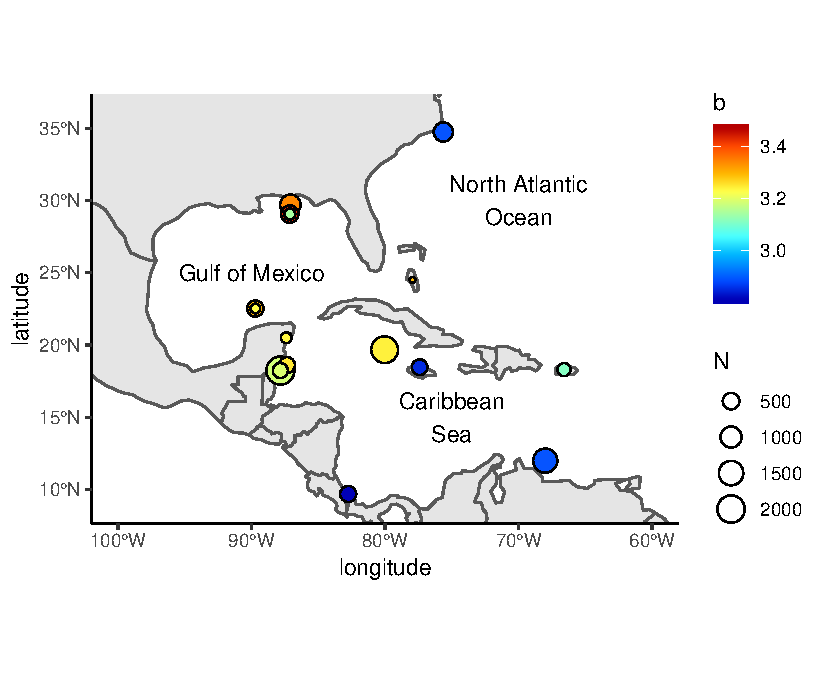
\includegraphics{Manuscript_files/figure-latex/unnamed-chunk-1-1.pdf}
\caption{\label{fig:map}Locations where allometric growth parameters of
lionfish (\emph{Pterois spp}) have been reported. Circle sizes indicate
sample size from each study, colors indicate the \(b\) coefficient from
Eq. \ref{eq:allometric}.}
\end{figure}

Parameters from the central Mexican Caribbean were obtained from data
collected in 10 sampling sites along the central Mexican Caribbean coast
in 2010 (Table S1). Sampling locations included wall and carpet reefs at
depths between 5.7 m and 38.1 m. All observed lionfish (n = 109) were
collected using hand nets and numbered collection bottles. The use of
hand nets prevented any weight loss due to bleeding and allowed better
representation of small sizes by eliminating gear selectivity. Organisms
were euthanized via pithing and Total Length (TL; mm) and Total Weight
(TW; g) were recorded before freezing organisms.

The weight at length relationship for lionfish in the central Mexican
Caribbean was calculated with the allometric growth function:

\begin{equation}
\label{eq:allometric}
TW = aTL^b
\end{equation}

Where \(a\) is the ponderal index and \(b\) is the scaling exponent or
allometric parameter. When \(b = 3\), it is said that the organism
exhibits a perfect isometric growth. Transforming this equation via
base-10 logarithms:

\begin{equation}
\label{eq:log-alo}
log_{10}(TW) = b\times log_{10}(TL) + log_{10}(a)
\end{equation}

This can be simplified and re-written as:

\begin{equation}
\label{eq:log-alo-trans}
Y = mX + c
\end{equation}

Where \(Y = log_{10}(TW)\), \(m = b\), \(X = log_{10}(TL)\), and
\(c = log_{10}(a)\). Since \(b = m\), we will only use \(b\) throughout
the paper for simplicity. The coefficients (\(c\) and \(b\)) were
estimated with an Ordinary Least Squares Regression and
heteroskedastic-robust standard error correction \citep{zeileis_2004}.
The \(b\) coefficient was tested against the null hypothesis of
isometric growth (\emph{i.e.} \(H_0: b = 3\)). Coefficients were tested
with a two-tailed Student's t, and the significance of the regression
was corroborated with an F-test.

Combining the length-weight parameters extracted from the literature and
the additional pair calculated here, we obtain a total of 18 pairs. We
test wether using \emph{ex situ} parameters produces differences in
weight estimates by estimating TW from the 109 length observations of
lionfish from the central Mexican Caribbean with each ot the 18
relationships. Predicted weights were divided by know observed weights
to obtain a simple measurement of over- or underestimation. Difference
in mean weight ratios across studies were tested with a one-way analysis
of variance (ANOVA). All analyses were performed in R version 3.5.0
\citep{rcore_2018}. Raw data and code used in this work are available at
dryad.org.

\section*{Results}

The model adjusted to Eq. \ref{eq:log-alo-trans} estimated the
coefficient values at \(b = 3.2347391\) and \(c = -5.4940866\)
(\(R^2 = 0.977\), F(df = 1; 107) = 6928.67, \(p < 0.001\)). The
allometric factor (\(b\)) was significantly different from the value of
isometric growth of \(b = 3\) (\(t(107) = 6.04; p<0.001\)), indicating
that lionfish present allometric growth. More information on model fit
is presented in TableS2. The relationship between TL and TW is presented
in Figure \ref{fig:l-w-carib}.

From this study in the central Mexican Caribbean and the 12
peer-reviewed studies that reported length-weight parameters for
\emph{P. volitans} 17 parameters were identified (Table
\ref{tab:all_params}, Fig \ref{fig:all_allo}). Two studies
\citep{aguilarperera_2016,fogg_2013} reported gender-level and pooled
parameters, while the rest presented pooled results. Reviewed studies
presented information for organisms obtained at depths between 0.5 and
57 m. Three studies explicitly stated that their organisms were sampled
with pole spears
\citep{aguilarperera_2016,chin_2016,dahl_2014,sabidoitz_2016}, and five
studies mentioned that some of their organisms were obtained with pole
spears (or other type of harpoon) but also hand-held nets or fish traps
\citep{sandel_2015,barbour_2011,fogg_2013,edwards_2014,sabidoitza_2016,sabidoitz_2016,toledohernndez_2014},
and two studies did not specify how organisms were sampled
\citep{deleon_2013,darling_2011}. \citet{fogg_2013} use spine-less
weight in the length-weight relationship estimation.

Parameters from models fit to males or females exclusively tend to have
a higher steepness (\emph{i.e.} higher allometric parameter), with mean
\(\pm\) standard deviation values of \(b = 3.27 \pm 0.06\) and
\(b = 3.31 \pm 0.23\) for males and females respectively, compared to
parameters from models for pooled genders with a mean \(\pm\) standard
deviation value of \(b = 3.14 \pm 0.20\). In the case of the ponderal
index (\(a\)) and its \(log_{10}\) transformation (\(c\)), values were
higher for parameters for pooled genders. Figure \ref{fig:all_allo}
shows the length-weight relationships with parameters from all studies.

There were significant differences in predicted-to-observed weight
ratios estimated for each pair of parameters (F(df = 15; 1728) = 38.26;
p \textless{} 0.001). From all allometric parameters reviewed, those of
\citet{sabidoitz_2016} in Banco Chinchorro, (Caribbean) provided the
lowest weight estimates, with a predicted-to-observed weight ratio of
0.80 \(\pm\) 0.19 (mean \(\pm\) SD). On the other hand,
\citet{barbour_2011} in the Northern Atlantic yielded the highest weight
estimates, with a mean (\(\pm\) SD) predicted-to-observed weight ratio
of 1.76 \(\pm\) 0.50. Predicted-to-observed weight ratios are presented
in Figure \ref{fig:bio_ratio}.

\begin{figure}
\centering
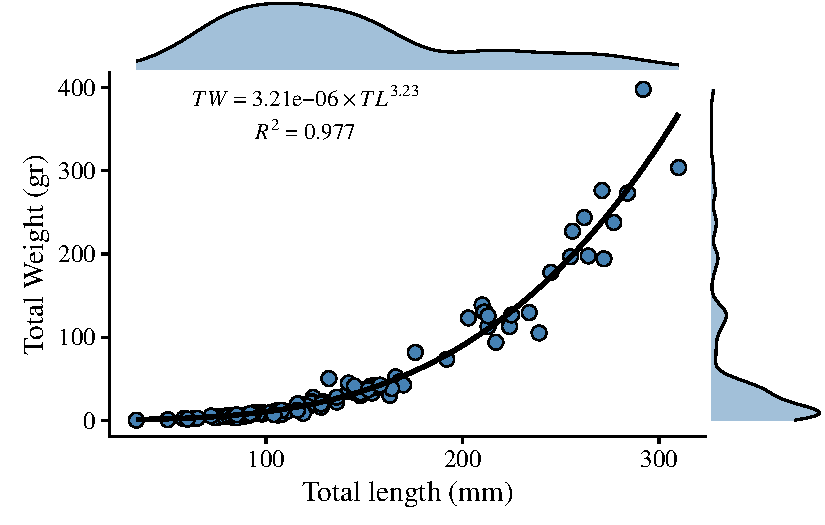
\includegraphics{Manuscript_files/figure-latex/unnamed-chunk-4-1.pdf}
\caption{\label{fig:l-w-carib}Length-weight relationship for 109
lionfish sampled in the central Mexican Caribbean. Points indicate
samples, dashed black line indicates curve of best fit, marginal plots
represent the density distribution of each variable.}
\end{figure}

\begin{table}

\caption{\label{tab:unnamed-chunk-5}\label{tab:all_params}Summary of 18 allometric growth parameters available for lionfish in the invaded range from peer-reviewed literature and this study. All parameters have been adjusted to convert from millimeters to grams. n = Sample size, Sex specifies whether data was presented for Females (F), Males (M), or both genders combined (B), a = scaling parameter for Eq. 1 (presented in $\times 10^{-5}$), c = y-intercept for Eq. 3, b = exponent or slope for Eq. 1 or Eq. 3, respectively. The $R^2$ column indicates reported model fit.}
\centering
\begin{tabular}[t]{llllrrll}
\toprule
Region & Sex & n & a & b & c & \$R\textasciicircum{}2\$ & Reference\\
\midrule
Caribbean & B & 458 & 3.6 & 2.81 & -4.44 & - & Sandel et al., 2015\\
Caribbean & B & 419 & 2.8 & 2.85 & -4.56 & 0.8715 & Chin et al., 2016\\
Caribbean & B & 1450 & 2.3 & 2.89 & -4.64 & 0.96 & de Leon et al., 2013\\
Caribbean & B & 1887 & 0.3 & 3.24 & -5.52 & 0.97 & Edwards et al., 2014\\
Caribbean & B & - & 0.25 & 3.29 & -5.60 & - & Darling et al., 2011\\
\addlinespace
Caribbean & B & 2143 & 0.52 & 3.18 & -5.28 & 0.9907 & Sabido-Itza et al., 2016\\
Caribbean & B & 227 & 0.8 & 3.11 & -5.10 & 0.958 & Toledo-Hernández et al., 2014\\
Caribbean & B & 449 & 0.23 & 3.25 & -5.64 & 0.97 & Sabido-Itza et al., 2016b\\
Caribbean & B & 368 & 0.32 & 3.19 & -5.50 & 0.98 & Sabido-Itza et al., 2016b\\
Caribbean & B & 109 & 0.32 & 3.23 & -5.49 & 0.9766 & This study\\
\addlinespace
GoM & B & 934 & 0.21 & 3.34 & -5.68 & 0.98 & Dahl \& Patterson, 2014\\
GoM & B & 472 & 0.29 & 3.30 & -5.54 & 0.95 & Aguilar-Perera \& Quijano-Puerto, 2016\\
GoM & F & 67 & 0.12 & 3.47 & -5.93 & 0.95 & Aguilar-Perera \& Quijano-Puerto, 2016\\
GoM & M & 59 & 0.42 & 3.23 & -5.38 & 0.95 & Aguilar-Perera \& Quijano-Puerto, 2016\\
GoM & B & 582 & 0.14 & 3.43 & -5.86 & 0.99 & Fogg et al., 2013\\
\addlinespace
GoM & M & 119 & 0.27 & 3.31 & -5.57 & 0.97 & Fogg et al., 2013\\
GoM & F & 115 & 0.68 & 3.14 & -5.17 & 0.94 & Fogg et al., 2013\\
NorthAtlantic & B & 774 & 2.9 & 2.89 & -4.54 & - & Barbour et al.,2011\\
\bottomrule
\end{tabular}
\end{table}

\begin{figure}
\centering
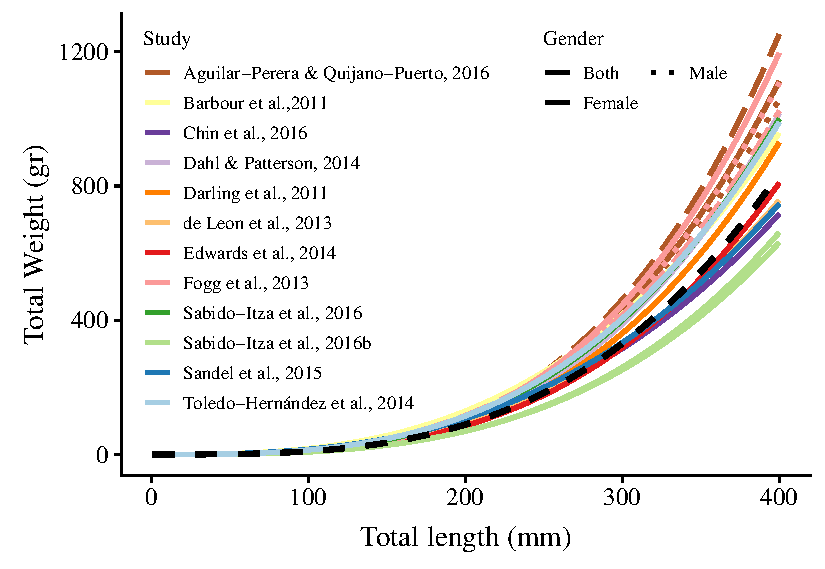
\includegraphics{Manuscript_files/figure-latex/unnamed-chunk-6-1.pdf}
\caption{\label{fig:all_allo}Length-weight relationships (n = 18) for 12
studies and this study. Colors indicate studies from which the
parameters were extracted. Solid lines indicate that the fit was
performed for males and females pooled together. Dotted lines indicate
that the regression was performed on females, and dashed lines indicate
it was performed for males. The dashed black line represents the
relationship estimated in this study.}
\end{figure}

\begin{figure}
\centering
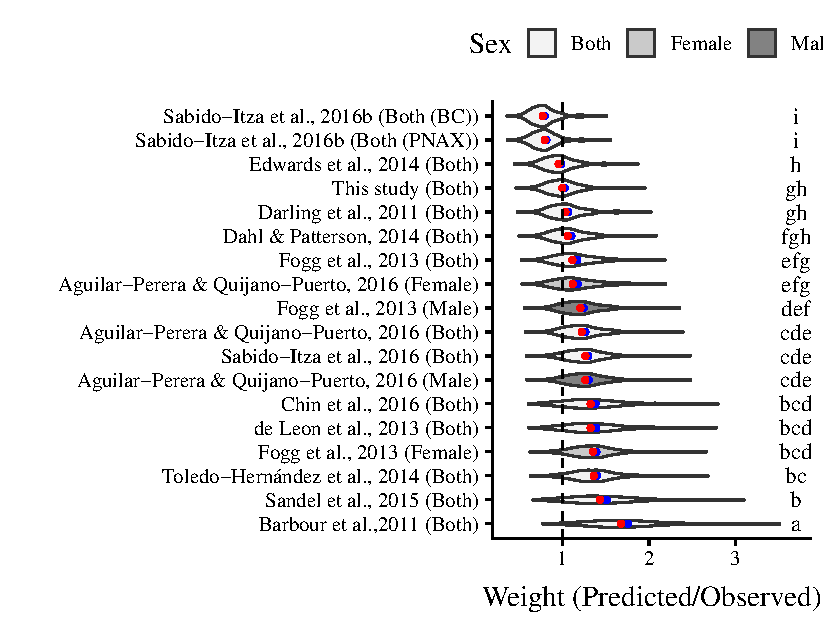
\includegraphics{Manuscript_files/figure-latex/unnamed-chunk-7-1.pdf}
\caption{\label{fig:bio_ratio}Violin plot showing the distribution of
predicted to observed weight ratios for 18 pairs of allometric
parameters. Red and blue circles indicate median and mean values,
respectively. Like letters indicate values that do not differ
significantly (Tukey's HSD; p \textless{} 0.05).}
\end{figure}

\clearpage

\section*{Discussion}

A new pair of allometric growth parameters for lionfish in the central
Mexican Caribbean are provided, complimenting existing literature for
other sites in the Mexican Caribbean
\citep{sabidoitza_2016,sabidoitz_2016}. Additionally, the study
identifies regional differences in length-weight relationships.

The length-weight coefficients estimated in this study were within the
range identified by studies in other regions (Table
\ref{tab:all_params}). However, the ones presented here provide lower
weight estimates for similar lenmgths. Until about TL = 200 mm, there
are no appreciable differences between the parameters for organisms from
the Mexican Caribbean and those for little Cayman \citep{edwards_2014}
and Jamaica \citep{chin_2016}. Yet, for larger organisms (TL
\textgreater{} 270 mm) parameters from Costa Rica \citep{sandel_2015}
and Bonaire \citep{deleon_2013} provide similar estimates to those from
this study. Conversely, these same studies tend to estimate higher
weights --as compared to the ones reported here-- for smaller organisms,
likely due to the lack of small organisms in the samples used to
estimate their parameters.

There are evident differences in weight-at-length between organisms from
the Caribbean and Gulf of Mexico / North-Western Atlantic. Weight
estimates with parameters from the Gulf of Mexico and North-Western
Atlantic tend to be higher than those from the Caribbean. Similar
regional variation has been reported for age-at-length relationships of
this species across the invaded region \citep{fogg_2015,edwards_2014},
or when comparing populations from the invasion and native ranges
\citep{pusack_2016}. These may be driven by genetic differences or
organisms being exposed to distinct environmental conditions. For
example, work on mitochondrial DNA has shown two distinct population
groups, identified as the ``Caribbean group'' and ``Northern Group''
\citep{betancurr_2011}. Alternatively, \citet{fogg_2015} suggest that
differences observed in age-at-length ``may bemore related to climate
rather than other biological and ecological factors''. Differences in
weight-at-length could also reflect differences in energy input
(\emph{i.e.} in some regions, lionfish eat more) or differential usage
of this energy (\emph{e.g.} regional differences in predator abundances
lead to different usage of energy), or a combination of both. Future
research should focus on identifying which occurs here.

The results presented in this paper can have major implications for
management. For example, \citet{edwards_2014} simulate lionfish culling
using parameters from North Carolina and Little Cayman, and identify
that the difference in time required for the population to recover to
90\% of its initial biomass after removals cease was of up to four
years. Our results show that, for a given length, using one set of
parameters or the other can result in a threefold increase in estimated
weight. This differences become especially relevant when estimating
biomass available for harvest, predicting effects on local ecosystems,
or evaluating the effectiveness of removal programs. Future research
should try to use, to the extent possible, parameters calculated for
their region, or use different parameters to provide upper and lower
bounds in their results. At the same time, this highlights the need for
more basic research that furthers our understanding of lionfish biology.
To better manage the invasion, we must perform research that can
describe biologically important information of lionfish throughout its
invasion range \citep{johnson_2016}.

\section*{Aknowledgements}

I would like to thank thank Nils Van Der Haar and Michael Doodey from
Dive Aventuras as well as Guillermo Lotz-Cador who provided help to
collect samples.

\bibliography{references}

\end{document}